\newcommand{\figuraModelosAtmosfericos}{%
\begin{figure}[htbp]
    \centering
    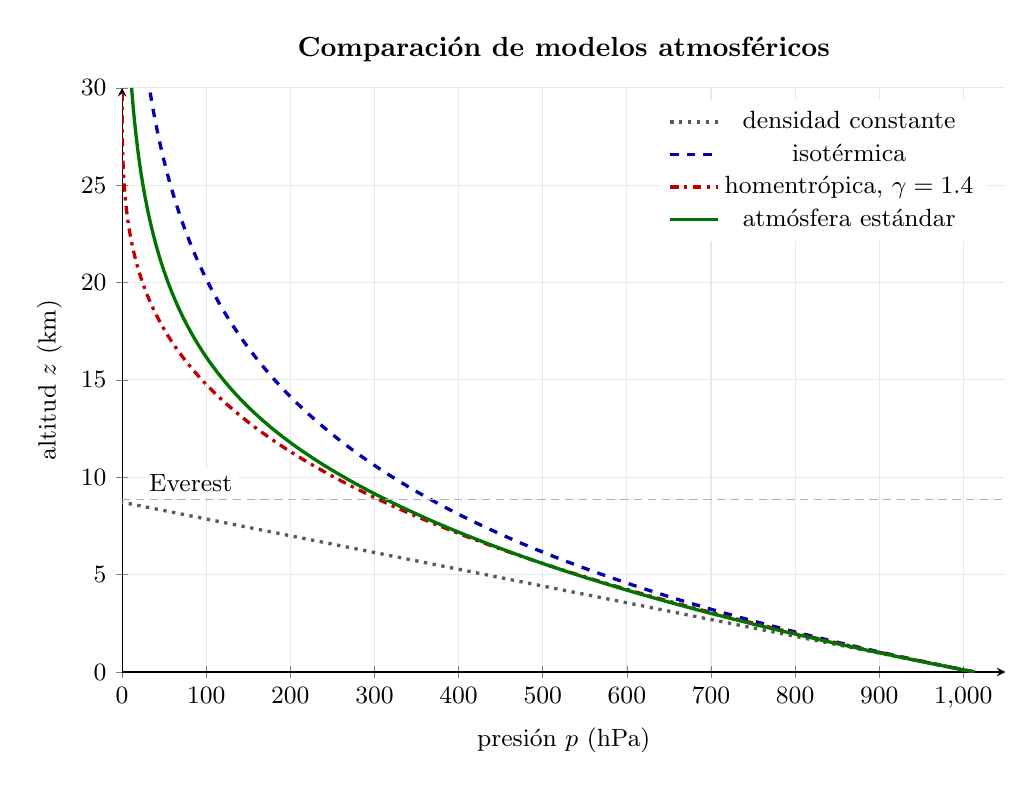
\begin{tikzpicture}[font=\small]
        \begin{axis}[
            width=12.8cm,
            height=9.0cm,
            xmin=0,
            xmax=1050,
            ymin=0,
            ymax=30,
            xlabel={presión $p$ (hPa)},
            ylabel={altitud $z$ (km)},
            axis lines=left,
            grid=major,
            major grid style={gray!18},
            legend style={
                at={(0.98,0.98)},
                anchor=north east,
                draw=none,
                fill=white,
                font=\small
            },
            title={Comparación de modelos atmosféricos},
            title style={font=\bfseries}
        ]
            \addplot[very thick,black!65,dotted,samples=120,domain=0:8.72]
                ({1013*(1-x/8.72)},x);
            \addlegendentry{densidad constante}

            \addplot[very thick,blue!70!black,dashed,samples=180,domain=0:30]
                ({1013*exp(-x/8.72)},x);
            \addlegendentry{isotérmica}

            \addplot[very thick,red!75!black,dash dot,samples=180,domain=0:30]
                ({1013*(1-x/30.52)^3.5},x);
            \addlegendentry{homentrópica, $\gamma=1.4$}

            \addplot[very thick,green!45!black,samples=140,domain=0:11]
                ({1013*(1-0.0065*x*1000/288.15)^5.2559},x);
            \addlegendentry{atmósfera estándar}
            \addplot[very thick,green!45!black,samples=140,domain=11:30,
                     forget plot]
                ({226.32*exp(-(x-11)/6.34)},x);

            \draw[densely dashed,gray!60]
                (axis cs:0,8.848)--(axis cs:1050,8.848);
            \node[anchor=south west,fill=white,inner sep=2pt]
                at (axis cs:25,8.95) {Everest};
        \end{axis}
    \end{tikzpicture}
    \caption{Presión atmosférica predicha por cuatro modelos. El modelo de
    densidad constante se anula a baja altitud; el isotérmico permanece
    exponencial; el homentrópico reproduce razonablemente la troposfera, pero
    se anula a una altura finita.}
    \label{fig:modelos-atmosfericos}
\end{figure}%
}